\documentclass[border=0pt]{standalone}

\usepackage{fontspec}
\setmainfont{texgyreheros}[Extension=.otf,UprightFont=*-regular,BoldFont=*-bold,ItalicFont=*-italic,BoldItalicFont=*-bolditalic]

\usepackage{tikz}
\usetikzlibrary{arrows.meta}
\newcommand{\labelat}[4]{\node[font=\fontsize{#3pt}{#3pt}\selectfont,inner sep=0pt,outer sep=0pt,align=center] at (#1,#2) {#4};}
\newcommand{\boldat}[3]{\labelat{#1}{#2}{8.6}{\bfseries #3}}
\begin{document}
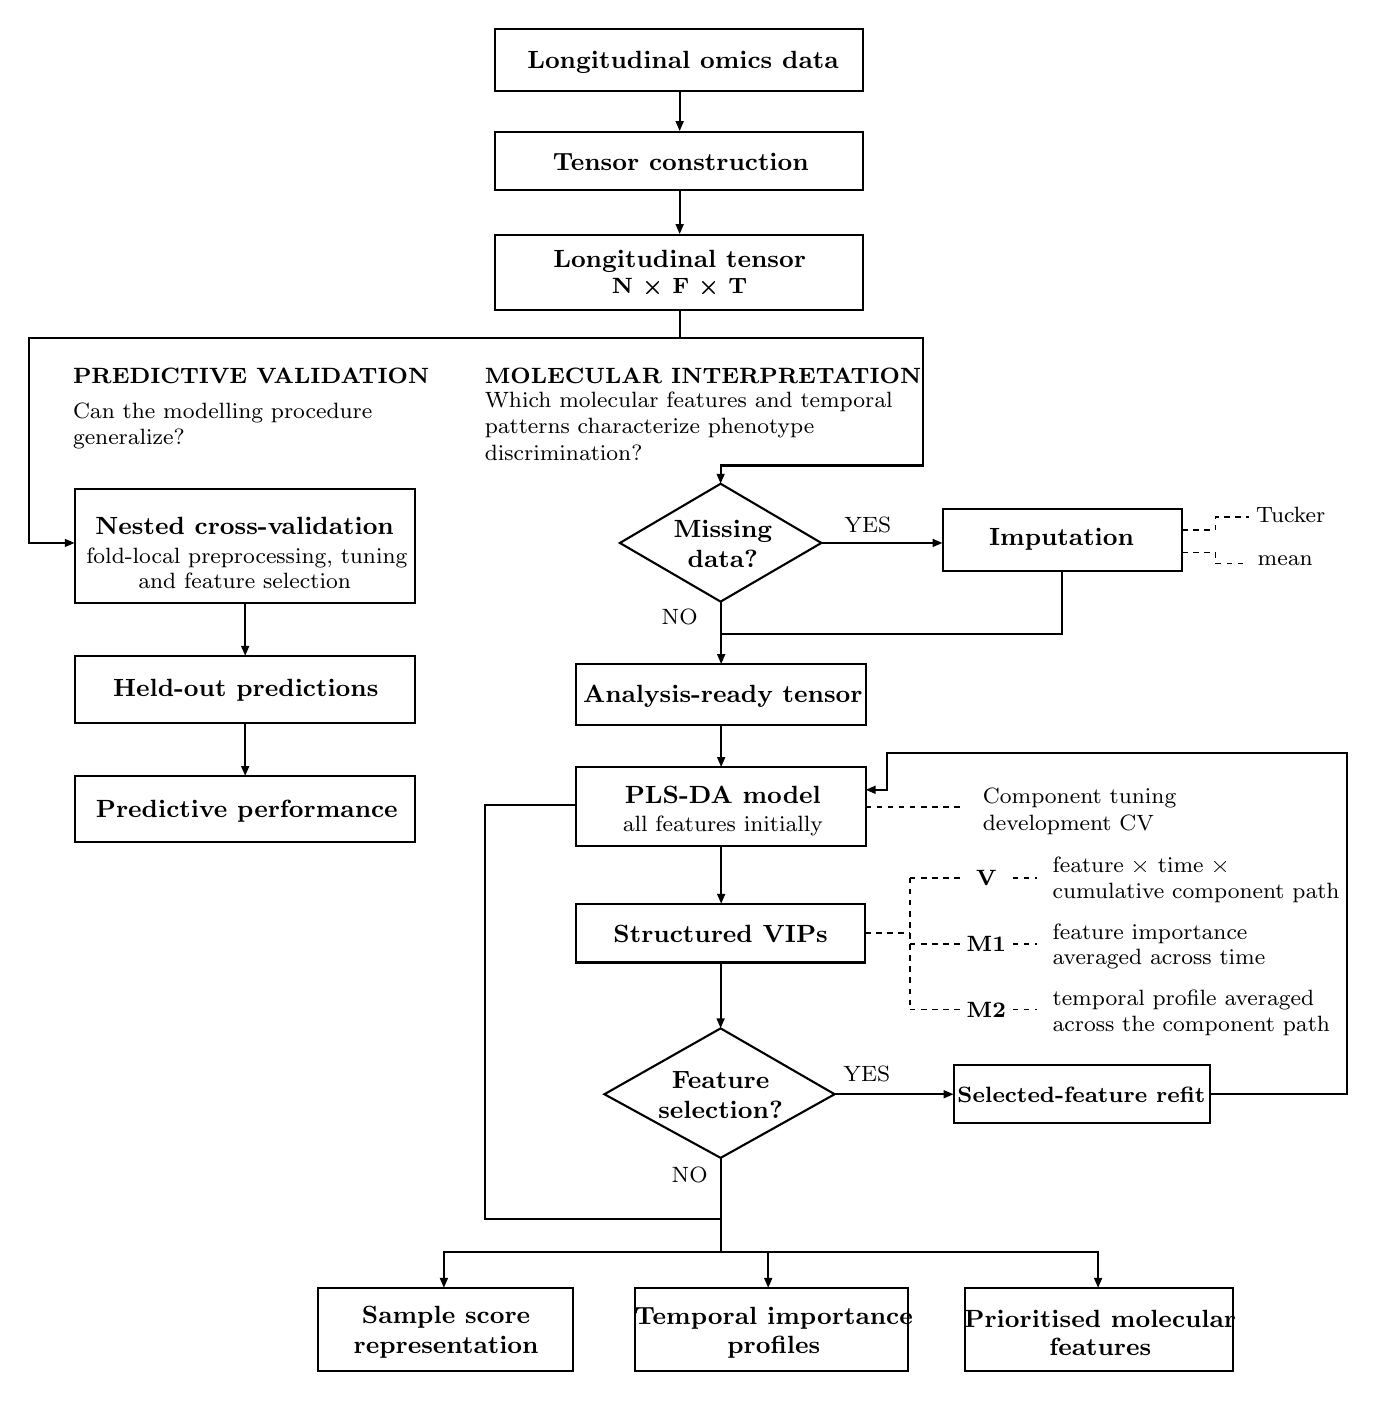
\begin{tikzpicture}[x=0.4pt,y=-0.4pt,line width=0.76pt,line join=miter,
  arr/.style={-{Triangle[length=3.6pt,width=2.8pt]}},
  annotationline/.style={dash pattern=on 2pt off 2pt,line width=0.6pt}]
\path[use as bounding box] (21,15) rectangle (1214,1241.754);
% Main core
\draw (443.5,16.5) rectangle (775.5,72.5);
\boldat{613}{46}{Longitudinal omics data}
\draw[arr] (610,72.5)--(610,108.5);
\draw (443.5,109) rectangle (775.5,162);
\boldat{611}{136}{Tensor construction}
\draw[arr] (610,162)--(610,201.5);
\draw (443.5,202.5) rectangle (775.5,270);
\labelat{610}{226}{8.6}{\bfseries Longitudinal tensor}
\labelat{610}{250}{8}{\bfseries N × F × T}
\draw (610.5,270)--(610.5,295.5);
% Branch division
\draw[arr] (610.5,295.5)--(22.5,295.5)--(22.5,480.5)--(63.5,480.5);
\draw[arr] (610.5,295.5)--(829.5,295.5)--(829.5,410.5)--(647,410.5)--(647,427);
\node[anchor=west,inner sep=0pt,font=\fontsize{8}{9.6}\selectfont\bfseries] at (61,330) {PREDICTIVE VALIDATION};
\node[anchor=west,inner sep=0pt,font=\fontsize{8}{9.6}\selectfont\bfseries] at (433,330) {MOLECULAR INTERPRETATION};
\node[anchor=west,inner sep=0pt,font=\fontsize{8}{9.6}\selectfont,align=left] at (61,375) {Can the modelling procedure\\generalize?};
\node[anchor=west,inner sep=0pt,font=\fontsize{8}{9.6}\selectfont,align=left] at (433,375) {Which molecular features and temporal\\patterns characterize phenotype\\discrimination?};
% Predictive branch.
\draw (63.5,432) rectangle (370.5,534.5);
\boldat{217}{465}{Nested cross-validation}
\labelat{219}{494}{8}{fold-local preprocessing, tuning}
\labelat{217}{515}{8}{and feature selection}
\draw[arr] (217.5,534.5)--(217.5,582.5);
\draw (63.5,582.5) rectangle (370.5,643);
\boldat{218}{614}{Held-out predictions}
\draw[arr] (217.5,643)--(217.5,691);
\draw (63.5,691) rectangle (370.5,750.5);
\labelat{219}{723}{8.6}{\bfseries Predictive performance}
% Missingness and imputation.
\draw (647,427)--(738,480.5)--(647,533.5)--(556,480.5)--cycle;
\boldat{649}{470}{Missing}
\boldat{649}{495}{data?}
\draw[arr] (738,480.5)--(847.5,480.5);
\labelat{780}{464}{8}{YES}
\draw (847.5,449.5) rectangle (1064,506);
\boldat{955}{477}{Imputation}
\draw[annotationline] (1064,469)--(1094,469)--(1094,457)--(1124,457);
\draw[annotationline] (1064,489)--(1094,489)--(1094,499)--(1124,499);
\labelat{1162}{455}{8}{Tucker}
\labelat{1157}{497}{8}{mean}
\draw (955.5,506)--(955.5,563)--(647.5,563);
\draw[arr] (647.5,533.5)--(647.5,590);
\labelat{610}{547}{8}{NO}
\draw (516.5,590) rectangle (778,645);
\labelat{649}{619}{8.6}{\bfseries Analysis-ready tensor}
\draw[arr] (647.5,645)--(647.5,683);
% Model, component tuning and VIP annotation.
\draw (516.5,683) rectangle (778,754);
\boldat{649}{708}{PLS-DA model}
\labelat{649}{736}{8}{all features initially}
\draw[annotationline] (778,719)--(865,719);
\node[anchor=west,inner sep=0pt,font=\fontsize{8}{9.6}\selectfont,align=left] at (883,723) {Component tuning\\development CV};
\draw[arr] (647.5,754)--(647.5,806.5);
\draw (516.5,806.5) rectangle (777.5,859.5);
\boldat{647}{834}{Structured VIPs}
\draw[annotationline] (777.5,833)--(818,833);
\draw[annotationline] (818,783)--(818,902);
\draw[annotationline] (818,783)--(863,783);
\draw[annotationline] (818,843)--(863,843);
\draw[annotationline] (818,902)--(863,902);
\labelat{887}{783}{8.4}{\bfseries V}
\labelat{887}{843}{8.4}{\bfseries M1}
\labelat{887}{902}{8.4}{\bfseries M2}
\draw[annotationline] (911,783)--(933,783);
\draw[annotationline] (911,843)--(933,843);
\draw[annotationline] (911,902)--(933,902);
\node[anchor=west,inner sep=0pt,font=\fontsize{8}{9.2}\selectfont,align=left] at (946,785) {feature × time ×\\cumulative component path};
\node[anchor=west,inner sep=0pt,font=\fontsize{8}{9.2}\selectfont,align=left] at (946,845) {feature importance\\averaged across time};
\node[anchor=west,inner sep=0pt,font=\fontsize{8}{9.2}\selectfont,align=left] at (946,905) {temporal profile averaged\\across the component path};
% Selection 
\draw[arr] (647,859.5)--(647,919);
\draw (647,919)--(750,978.5)--(647,1036)--(542,978.5)--cycle;
\boldat{647}{966}{Feature}
\boldat{647}{993}{selection?}
\draw[arr] (750,978.5)--(857.5,978.5);
\labelat{779}{960}{8}{YES}
\draw (857.5,952.5) rectangle (1089,1004.5);
\labelat{973}{979}{8}{\bfseries Selected-feature refit}
\draw[arr] (1089,978.5)--(1213,978.5)--(1213,670)--(797.5,670)--(797.5,703.5)--(778,703.5);
\draw (647,1036)--(647,1121);
\labelat{619}{1051}{8}{NO}
\draw (516.5,717.5)--(434.5,717.5)--(434.5,1091)--(647,1091);
\draw[arr] (647,1121)--(397,1121)--(397,1153.5);
\draw[arr] (647,1121)--(690,1121)--(690,1153.5);
\draw[arr] (690,1121)--(988,1121)--(988,1153.5);
% Outputs.
\draw (283.5,1153.5) rectangle (513.5,1228.5);
\boldat{399}{1180}{Sample score}
\boldat{399}{1207}{representation}
\draw (570,1153.5) rectangle (816,1228.5);
\boldat{695}{1181}{Temporal importance}
\boldat{695}{1207}{profiles}
\draw (868,1153.5) rectangle (1110,1228.5);
\boldat{990}{1181}{Prioritised molecular}
\boldat{990}{1207}{features}
\end{tikzpicture}
\end{document}

